% Basic setup
\documentclass[12pt,a4paper]{article} % Defines the document type as an article with 12pt font size on A4 paper.

% Importing packages
\usepackage[english]{babel} % Sets the document language to English, adjusting hyphenation and language-specific typographic rules.
\usepackage[lmargin=2.5cm,rmargin=2.5cm,tmargin=2.5cm,bmargin=2.5cm]{geometry} % Sets custom page margins: left/right 2.5cm, top 2.5cm, bottom 2.5cm.

% Loading packages
\usepackage{amsmath}
\usepackage{hyperref}    % Enables hyperlinks for references, URLs, and citations.
\usepackage{xcolor}      % Provides tools for defining and using colors.
\usepackage{graphicx}    % Allows inclusion of images and graphics.
\usepackage{caption}     % Customizes captions for figures and tables.
\usepackage{subcaption}  % Supports subfigures and subcaptions within figures.
\usepackage{minted}      % Enables syntax highlighting for code listings.
\usepackage[T1]{fontenc} % Ensures proper font encoding, important for correct character rendering. Don't touch this.
\usepackage{lmodern}     % Sets the font to something more modern and easy to read.
\usepackage{setspace}    % Provides control over line spacing.
\usepackage{csquotes}    % Improves handling of quotations.
\usepackage{setspace}    % Used to set line spacing
\usepackage{longtable,booktabs,array} % Packages for advanced table formatting.
\usepackage{wasysym}
\usepackage[
  backend=biber,
  style=apa,  
]{biblatex}  % Manages citations and bibliography with APA style.

\setstretch{1.5} % Sets line spacing

\definecolor{LightGray}{gray}{0.9}  % Defines a custom color 'LightGray' with 90% gray, used for the code block background.
\hypersetup{                        % Configures hyperlink colors and behavior.
  colorlinks=true,                  % Enable colored links instead of boxes.
  linkcolor={blue},                 % Sets link color to blue.
  filecolor={maroon},               % Sets file link color to maroon.
  citecolor={blue},                 % Sets citation link color to blue.
  urlcolor={blue}}                  % Sets URL link color to blue.

\addbibresource{assets/bib-template.bib} % Adds the bibliography file.

\title{Place Holder page titre}        % Sets the document title.
\makeatletter
\providecommand{\subtitle}[1]{%     % Custom command to add a subtitle.
  \apptocmd{\@title}{\par {\large #1 \par}}{}{}
}

\makeatother
\subtitle{Va être remplacée par celle sur Teams}  % Sets the document subtitle.
\author{Charles Bouthillier Paul Charvet William Hamilton Samuel Roy}% Sets the author's name.
\date{2025-12-12}                   % Sets the document date.

% \renewcommand{\familydefault}{\sfdefault} % Changes the default font to one without serifs

% From this point, the preamble ends and the actual content of the document starts.
\begin{document}
\pagenumbering{gobble} % Stops counting the pages from this point until changed again.
\maketitle
%\begin{abstract}
%This is the LaTeX template (\textbf{Version 1.1}) from the DH Lab of the University of Basel. It is suitable for Seminar Papers and Master's / PhD theses, but can be adapted to fit a variety of use cases. It was created by Stefan Freitag and is derived from the Quarto template, which is also available from the DH Lab.

%The abstract of your paper / thesis goes right here. It will appear on the cover sheet (very first page) of the PDF, together with the title, subtitle, author name and date.

%If you do not want your document to have an abstract, you can also simple delete the 'abstract' part (or comment it out) with all its content and the final document will be created without it.
%\end{abstract}
\begin{center}
    \vfill
    \begin{figure}[H] 
          \includegraphics[width=.8\linewidth]{./assets/Université_Laval_logo_et_texte.svg.png}
    \end{figure}
        \setcounter{figure}{0}
        
    Université Laval\\
    Facutlé de science génie\\
    Québec
\end{center}
\newpage
\renewcommand*\contentsname{Table des matières} % This controls the title of your table of contents.
{
\hypersetup{linkcolor=}
\setcounter{tocdepth}{5} % Sets the maximum sublevel to be displayed within the table of contents.

\tableofcontents
}
\newpage
\pagenumbering{arabic}\setstretch{1.5} % Overwrites the previous command, pages are counted as normal from this point.


\section{Vue CAD 3D explosée}
    \begin{figure}[H] 
	    \includegraphics[width=1.1\linewidth]{./assets/Explose.png}
    \end{figure}

\section{captures d'écran des enveloppes d'impression}

\subsection{Volumes Préférentiels X-Y}
    \subsubsection{Lot \#1}    
    \begin{figure}[H] 
	    \includegraphics[width=1.1\linewidth]{./assets/XY_pref1.pdf}
    \end{figure}
    \subsubsection{Lot \#2}
    \begin{figure}[H] 
	    \includegraphics[width=1.1\linewidth]{./assets/XY_pref2.pdf}
    \end{figure}

\subsection{Volumes Préférentiels Z} 
    \subsubsection{Lot \#3}    
    \begin{figure}[H] 
	    \includegraphics[width=1.1\linewidth]{./assets/Z_pref1.pdf}
    \end{figure}
    \subsubsection{Lot \#4}
    \begin{figure}[H] 
	    \includegraphics[width=1.1\linewidth]{./assets/Z_pref2.pdf}
    \end{figure}

\section{Croquis à main levé}

    \subsection{Concept \#1: Charles Bouthillier}
    \begin{figure}[H] 
	    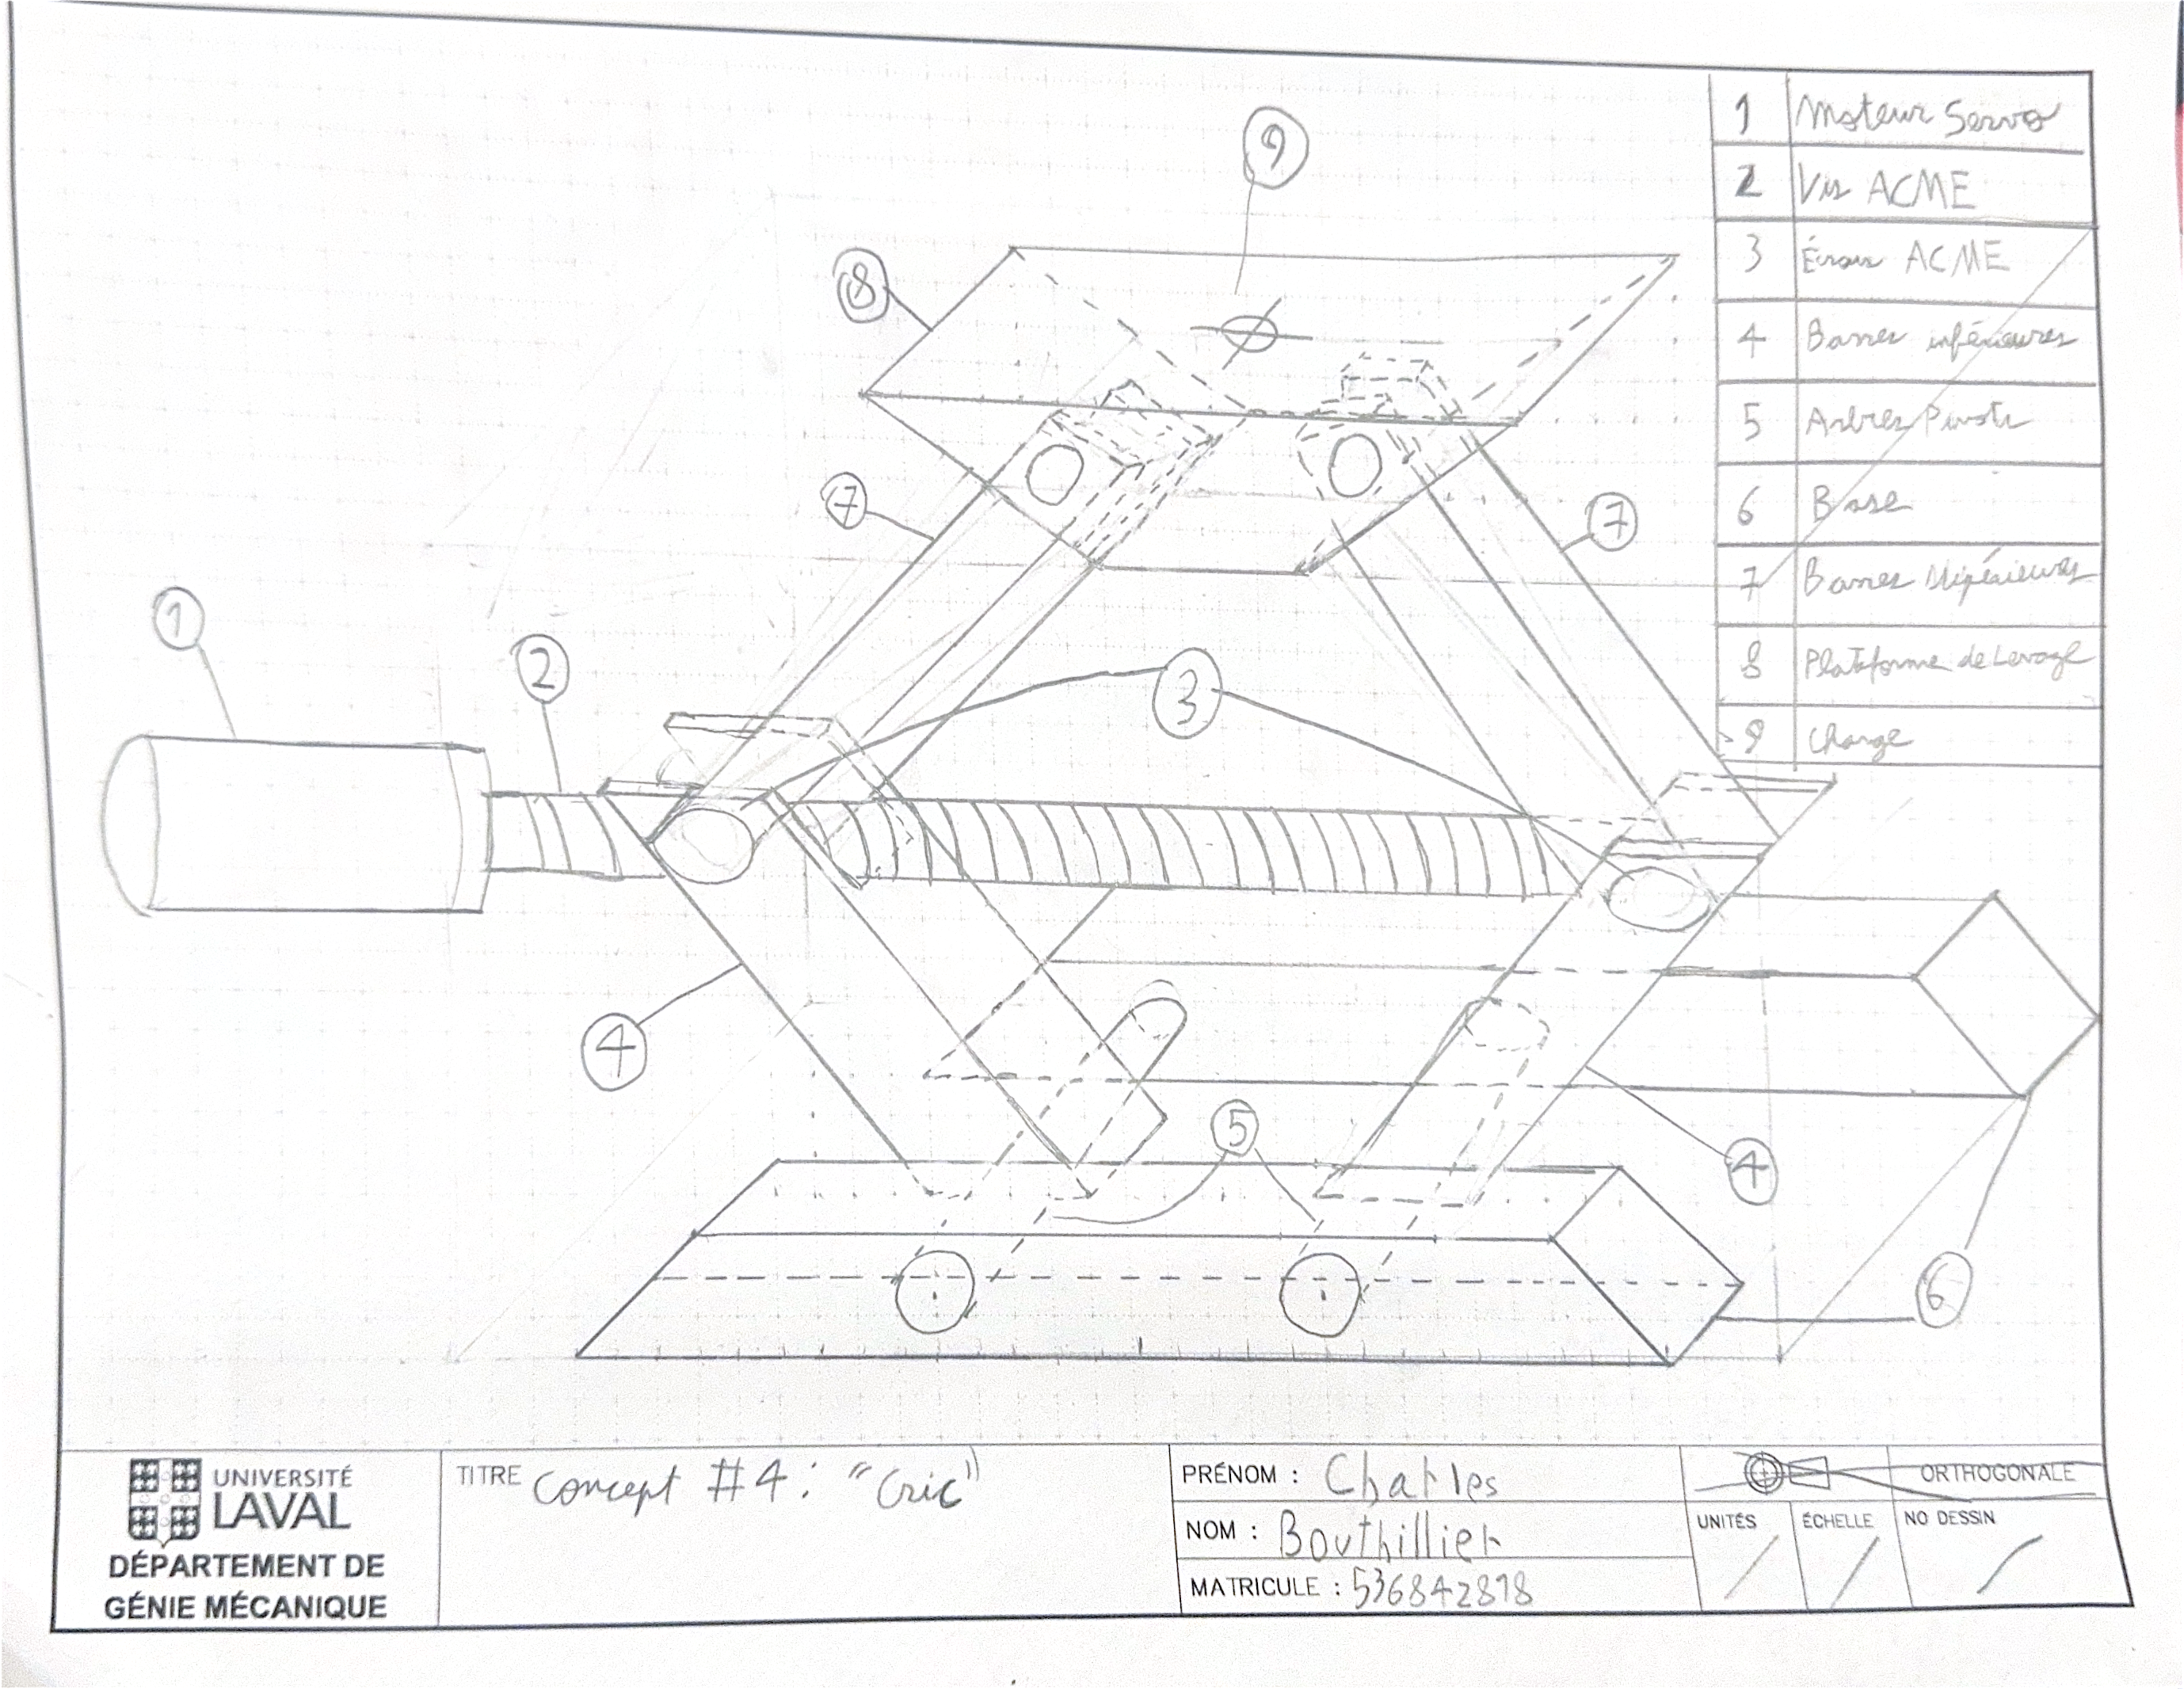
\includegraphics[width=1.1\linewidth]{./assets/Croquis_CB.pdf}
    \end{figure}
    \begin{par}
	    Explication du concept: Cette solution est inspiré d'un "cric" permettant de soulever des voitures. Le moteur (\#1) fait tourner une vis ACME (\#2). Deux écrous (\#3) sont bloqués en rotation sur la vis, lorsque le moteur tourne, ils seront naturellement pousser vers le centre de la vis, entrainant avec eux les pivots centraux des barres (\#4 et \#7). Lorsque les pivots centraux se rapprochent, les systèmes de barres se dressent, ce qui a pour efffet d'élever la plateforme (\#8), et par extension, la charge (\#9) qui y est posée.
    \end{par}
    \begin{figure}[H] 
	    \includegraphics[width=0.45\linewidth]{./assets/Signatures/Signature_CB.png}
    \end{figure}

    \subsection{Concept \#2: Samuel Roy}
    \begin{figure}[H] 
	    \includegraphics[width=1.1\linewidth]{./assets/Croquis_SR.pdf}
    \end{figure}
    \begin{par}
	    Explication du concept:
	    Voir image ci-dessus
    \end{par}
    \begin{figure}[H] 
	    \includegraphics[width=0.45\linewidth]{./assets/Signatures/Signature_SR.png}
    \end{figure}

    \subsection{Concept \#3: Paul Charvet}
    \begin{figure}[H] 
	    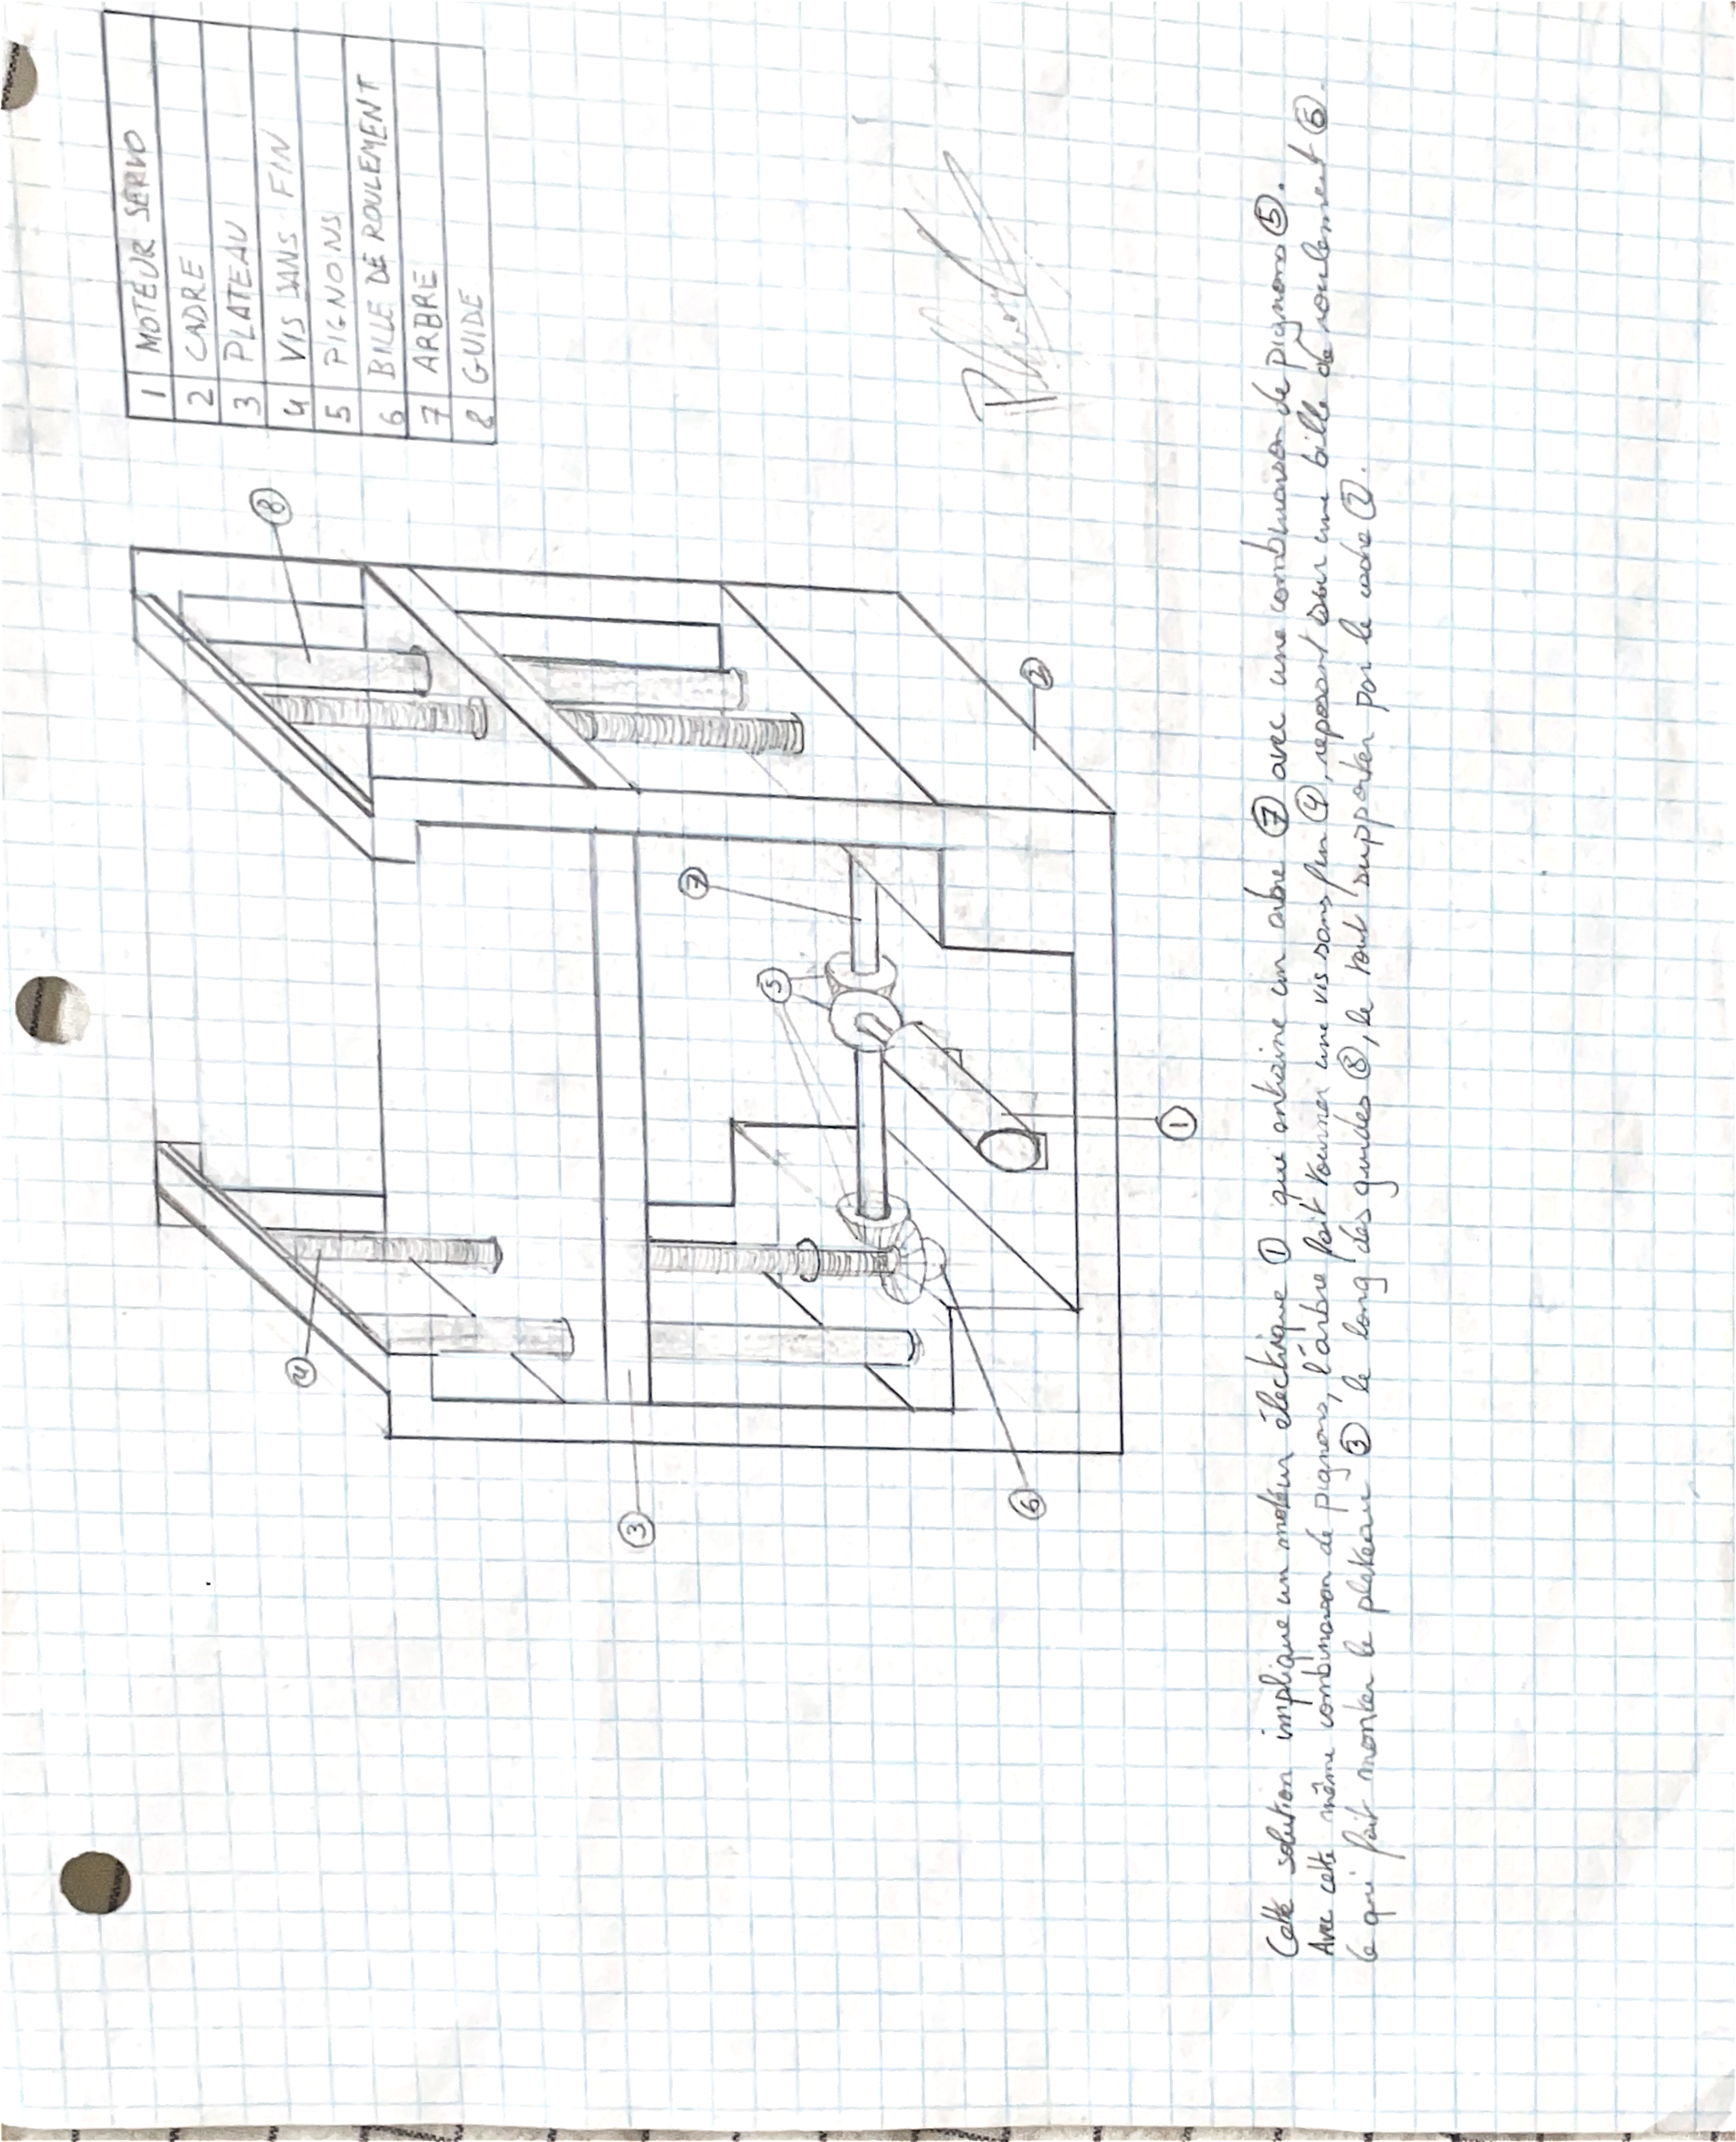
\includegraphics[width=1.1\linewidth]{./assets/Croquis_PC.pdf}
    \end{figure}
    \begin{par}
	    Explication du concept: Cette solution implique un moteur électrique (\#1) qui entraine un arbre (\#7) avec une combinaison de pignons (\#5). À l'aide de cette dernière, l'arbre fait tourner une vis sans fin (\#4) reposant sur une bille de roulement (\#6), ce qui fait monter le plateau (\#3) le long des guides (\#8), le tout supporter par le cadre (\#2). 
    \end{par}
    \begin{figure}[H] 
	    \includegraphics[width=0.30\linewidth]{./assets/Signatures/Signature_PC.png}
    \end{figure}

    \subsection{Concept \#4: William Hamilton}
    \begin{figure}[H] 
	    \includegraphics[width=1.1\linewidth]{./assets/Croquis_WH.pdf}
    \end{figure}
    \begin{par}
	    Explication du concept
    \end{par}
    \begin{figure}[H] 
	    \includegraphics[width=0.45\linewidth]{./assets/Signatures/Signature_WH.png}
    \end{figure}

    \subsection{Grille de sélection}
    \begin{figure}[H] 
	    \includegraphics[width=1.1\linewidth]{./assets/Grille.png}
    \end{figure}
    \subsection{Justification des cotes}
    \begin{par}
Pour le concept \#1, nous avons décidé d’attribuer la note de 60/100 au critère de propension à soulever une charge importante, en raison des contraintes susceptibles d’être appliquées aux pièces 5, dites « arbres pivots », lesquelles pourraient avoir des difficultés à les supporter.
Concernant la variabilité du niveau de charge pouvant être soulevée en fonction de la géométrie, nous estimons que, lorsque le système se rapproche de sa hauteur maximale, la répartition des contraintes est amenée à évoluer. Bien que nous n’ayons pas réalisé d’analyse approfondie, nous avons choisi d’attribuer une note de 80/100.
La complexité du mécanisme ainsi que le nombre de pièces ont été jugés raisonnables ; c’est pourquoi une note de 80/100 a été retenue pour ce critère.
Enfin, le niveau d’incertitude a également obtenu cette note, dans la mesure où il s’agit d’un concept déjà connu et couramment utilisé.
    \end{par}
\vspace{\baselineskip}
    \begin{par}
Pour le concept \#2, nous avons estimé que la capacité à soulever une charge importante serait limitée et que le couple requis atteindrait rapidement une valeur susceptible de bloquer le moteur. De plus, l’engrenage 5 risquerait de frotter contre le fond du boîtier. Pour ces raisons, nous avons attribué une note de 65/100.
Ensuite, bien que nous n’ayons réalisé ni calculs ni analyses détaillées, nous avons supposé que la hauteur du système n’influencerait pas sa capacité à soulever différentes charges. Ainsi, une note de 100/100 a été attribuée pour ce critère.
En ce qui concerne la complexité et le nombre de pièces, ce concept est de loin le plus simple ; la note de 95/100 lui a donc été accordée. Les cinq points retirés s’expliquent par la conception des pièces 2 et 5, respectivement la « worm gear » et la « wheel gear », jugée plus exigeante.
Enfin, une note de 70/100 a été attribuée en raison des incertitudes liées au système de transmission de puissance ainsi que du risque de flambage de la pièce 4, la « structure de guidage ».
    \end{par}
\vspace{\baselineskip}
    \begin{par}
Le concept \#3 a été jugé capable de soulever une charge importante, avec une note de 80/100, en raison de la présence de deux pièces 4, des « vis sans fin ». Toutefois, un travail d’optimisation des rapports de transmission aurait été nécessaire afin de garantir une meilleure capacité de reprise de charge.
Nous estimons que ce concept est parfaitement capable de supporter la charge indépendamment de la hauteur de la pièce 3, le « plateau », grâce aux pièces 8, les « guides ». C’est pourquoi la note de 100/100 a été attribuée pour ce critère.
En revanche, ce concept présente une complexité élevée, avec un grand nombre de pièces en mouvement, ce qui justifie la note de 30/100.
Enfin, concernant le niveau d’incertitude et de risque associé à ce concept, celui-ci a été jugé relativement faible. En effet, le système est très stable grâce aux guides et à la pièce 2, le « cadre », et une part importante des efforts est reprise par des pièces métalliques (4 et 6).
    \end{par}
\vspace{\baselineskip}
    \begin{par}
Pour le concept \#4, nous estimons que, bien qu’il soit très résistant, il présente un problème similaire à celui du concept 2, à savoir une variation de rapport de transmission insuffisante, susceptible d’entraîner le blocage du moteur. Une note de 70/100 a donc été attribuée.
En ce qui concerne la capacité de levage en fonction de la hauteur, nous avons jugé que l’impact serait limité ; c’est pourquoi une note de 90/100 a été accordée.
Nous avons également estimé que ce concept était peu complexe, car il comporte un nombre relativement réduit de pièces.
Enfin, nous avons considéré que la géométrie conique conférait une robustesse accrue au système, réduisant ainsi le risque de rupture.
    \end{par}
\section{Calculs}

\subsection{Calcul de faisabilité (\#1)}
	\subsubsection{DCL des composantes dans le chemin de force}	
\begin{enumerate}
\renewcommand{\labelenumi}{\alph{enumi})}
  \begin{minipage}{\linewidth}
  \item
  Moteur

  \medskip
  \includegraphics[width=1\linewidth]{./assets/DCL/Moteur.png}
  \end{minipage}
  \begin{minipage}{\linewidth}
  \item
  Vis sans fin

  \medskip
  \includegraphics[width=1\linewidth]{./assets/DCL/Worm.png}
  \end{minipage}
  \begin{minipage}{\linewidth}
  \item
  Roue dentée

  \medskip
  \includegraphics[width=1\linewidth]{./assets/DCL/Gear1.png}
  \end{minipage}
  \begin{minipage}{\linewidth}
  \item
  arbre au centre de la roue dentée

  \medskip
  \includegraphics[width=0.75\linewidth]{./assets/DCL/Shaft.png}
  \end{minipage}
  \begin{minipage}{\linewidth}
  \item
  Pignon 

  \medskip
  \includegraphics[width=1\linewidth]{./assets/DCL/Gear2.png}
  \end{minipage}
  \begin{minipage}{\linewidth}
  \item
  Écrou ACME

  \medskip
  \includegraphics[width=1\linewidth]{./assets/DCL/ACME_nut.png}
  \end{minipage}
  \begin{minipage}{\linewidth}
  \item
  Vis ACME

  \medskip
  \includegraphics[width=0.7\linewidth]{./assets/DCL/ACME_screw.png}
  \end{minipage}
\end{enumerate}
	\subsubsection{couple pour soulever 295,5kg}
\begin{center}
	\begin{tabular}{|c c c|}
		\hline
		Paramètre & symbole & valeur de base\\
		\hline
		masse à soulever & $M_{charge}$ & 295,5 [kg]\\
	constante de gravité & g & 9,81 [ \[m\,s^{-2}} \] ]\\
	pas de la vis ACME & P & 0,00254 [m]\\
	Diamètre primitif vis ACME & $\diameter_s$ & 0,011285 [m]\\
	lead angle & $\lambda$ & N/A [$\circ$]\\
	angle d'hélice & $\psi$ & 4,098 [$\circ$]\\
	coeff. friction vis-écrou & $\mu$ & 0,5 [-]\\
	coeff. friction nylon-nylon & f & 0,25 [-]\\
	efficacité & $\varepsilon$ & N/A [-]\\
	Torque pour soulever la charge & $T_c$ & N/A [Nm]\\
	rayon primitif du pinion & $R_g$ & 0,01915 [m]\\
	Perte de torque en friction au pinion & $T_f$ & N/A [Nm]\\
	Torque au pinion & $T_a$ & N/A [Nm]\\
	nombre de dents du pinion & $Z_a$ & 29 [-]\\
	nombre de dents de la roue dentée & $Z_b$ & 53 [-]\\
	efficacité engrenage hélicoïdal & $\eta$ & 0,98 [-]\\
	angle de pression & $\phi_n$ & 20 [$\circ$]\\
	efficacité engrenage vis sans fin & $e_w$ & N/A [-]\\
	nombre de filets vis sans fin & $Z_w$ & 2 [-]\\
	Couple du moteur & $C_{mot}$ & N/A [Nm]\\

		\hline
	\end{tabular}
\end{center}
\begin{enumerate}
  \renewcommand{\labelenumi}{\alph{enumi})}

  \item Torque pour soulever la charge
\[ \lambda = atan(\frac{P}{\pi*\diameter_s}) = 4,098 \]

\[ \varepsilon = \frac{tan(\psi)}{tan(\psi+atan(\mu))} = 0,1208 \]

\[ T_c = \frac{M_{charge}*g*P}{2\pi*\varepsilon} = 9,7 \]
  \item Transmission de torque entre la roue dentée et le pinion
	  \[ T_f = \frac{1}{2}f*M_{charge}*g*R_g=6,94 \]
\[ T_a = T_f+ T_c = 16,64  \]
\[ T_b = \eta*\frac{Z_b}{Z_a}*T_a = 29,21 \]
  \item Transmission de torque entre la roue dentée et la vis sans fin
\[ e_w = \frac{cos(\phi_n) - f*tan(\psi)}{cos(\phi_n) + f*cot(\psi)} = 0,18388 \]
\[ C_{mot} = T_{worm} = \frac{T_b*Z_w}{e_w*Z_b} = 6 > 1,2 Nm \]
Couple trop grand, il faut diminuer la charge sur le système
\end{enumerate}
	\subsubsection{couple pour soulever une charge optimale (34/75 kg/lbs}
\begin{center}
	\begin{tabular}{|c c c|}
		\hline
		Paramètre & symbole & valeur de base\\
		\hline
		masse à soulever & $M_{charge}$ & 34 [kg]\\
		\hline
	\end{tabular}
\end{center}

\begin{enumerate}
  \renewcommand{\labelenumi}{\alph{enumi})}

  \item Torque pour soulever la charge
	  \[ T_c = \frac{M_{charge}*g*P}{2\pi*\varepsilon} = 1,114 \]
  \item Transmission de torque entre la roue dentée et le pinion
	  \[ T_f = \frac{1}{2}f*M_{charge}*g*R_g=0,797 \]
\[ T_a = T_f+ T_c = 1,911  \]
\[ T_b = \eta*\frac{Z_b}{Z_a}*T_a = 3,354 \]
  \item Transmission de torque entre la roue dentée et la vis sans fin
\[ C_{mot} = T_{worm} = \frac{T_b*Z_w}{e_w*Z_b} = 0,689 < 1,2 Nm \]
\end{enumerate}
	\subsubsection{masse pour un couple moteur unitaire}
\begin{center}
	\begin{tabular}{|c c c|}
		\hline
		Paramètre & symbole & valeur de base\\
		\hline
		couple moteur & $C_{mot}$ & 1 [Nm]\\
		masse à soulever & $M_{charge}$ & N\A [kg]\\
		\hline
	\end{tabular}
\end{center}
\begin{enumerate}
  \renewcommand{\labelenumi}{\alph{enumi})}
  \item Transmission de torque entre le moteur et la roue dentée
\[ T_{w} = C_{mot} = 1 \]
\[ T_{b} = \frac{T_w*e_w*Z_b}{Z_w}= 4,8728 \]
  \item Transmission de torque entre la roue dentée et le pinion
\[ T_a = \frac{1}{\eta}*\frac{Z_a}{Z_b}*T_b = 2,72 \]
\[ T_c = T_a - T_f\]
  \item Torque pour soulever la charge
	  \[ M_{charge} = \frac{(T_a-T_f)*2\pi*\varepsilon}{g*P} \]

	  \[ M_{charge} = \frac{(T_a-\frac{1}{2}f*M_{charge}*g*R_g)*2\pi*\varepsilon}{g*P} \]

	  \[ M_{charge} = \frac{2*T_a*\pi*\varepsilon}{g*(P+f*R_g*\pi*\varepsilon)} = 48,30 kg \]

\end{enumerate}

	\subsubsection{temps de montée}
\begin{center}
	\begin{tabular}{|c c c|}
		\hline
		Paramètre & symbole & valeur de base\\
		\hline
		vitesse du moteur & $N_{mot}$ & 233 [rpm]\\
		nombre de filets de la vis sans fin & Z_w & 2 [-]\\
		nombre de dents de la roue dentée & Z_b & 53 [-]\\
		vitesse de la roue dentée & \omega_b & N/A [rpm]\\
		nombre de dents du pinion & Z_a & 29 [-]\\
		vitesse dy pinion & \omega_a & N/A [-]\\
		distance de levage & d & 0,04 [m]\\
		Pas de la vis ACME & P & 0,00254 [m]\\
		temps de levage & t_{montée} & N/A [s]\\
		\hline
	\end{tabular}
\end{center}
\[ \omega_b = \frac{N_{mot}*Z_w}{Z_b} = 8,79 \]

\[ \omega_a = \frac{\omega_{b}*Z_b}{Z_a} = 16,069 [RPM] = 0,268 [Hz] \]

\[ t_{montée} = \frac{d}{\omega_{a}*P} = 58,8 < 60 \]


\begin{center}
	\begin{tabular}{|c c c|}
		\hline
		Paramètre & symbole & valeur de base\\
		\hline
		couple moteur & $C_{mot\_boost}$ & 2,2 [Nm]\\
		masse à soulever & $M_{surcharge}$ & N/A [kg]\\
		\hline
	\end{tabular}
\end{center}

\subsubsection{Évaluer la surcharge}
\begin{center}
	\begin{tabular}{|c c c|}
		\hline
		Paramètre & symbole & valeur de base\\
		\hline
		couple moteur & $C_{mot\_boost}$ & 2,2 [Nm]\\
		masse à soulever & $M_{surcharge}$ & N/A [kg]\\
		\hline
	\end{tabular}
\end{center}
\begin{enumerate}
  \renewcommand{\labelenumi}{\alph{enumi})}
  \item Transmission de torque entre le moteur et la roue dentée
\[ T_{w} = C_{mot\_boost} = 2,2 \]
\[ T_{b} = \frac{T_w*e_w*Z_b}{Z_w}= 10,72 \]
  \item Transmission de torque entre la roue dentée et le pinion
\[ T_a = \frac{1}{\eta}*\frac{Z_a}{Z_b}*T_b = 5,984 \]
\[ T_c = T_a - T_f\]
  \item Torque pour soulever la charge
	  \[ M_{surcharge} = \frac{(T_a-T_f)*2\pi*\varepsilon}{g*P} \]

	  \[ M_{surcharge} = \frac{(T_a-\frac{1}{2}f*M_{surcharge}*g*R_g)*2\pi*\varepsilon}{g*P} \]

	  \[ M_{surcharge} = \frac{2*T_a*\pi*\varepsilon}{g*(P+f*R_g*\pi*\varepsilon)} = 106,26 kg \]

\end{enumerate}
\begin{table}[h]
\caption{Spécifications du système}
\begin{center}
	\begin{tabular}{|c c c|}
		\hline
		Paramètre & symbole & valeur de base\\
		\hline
		couple moteur d'opération & $C_{mot}$ & 0,689 [Nm]\\
		masse admissible & $M_{charge}$ & 34 [kg]\\
		vitesse du moteur & $N_{mot}$ & 233 [rpm]\\
		temps de levage & $t_{montée}$ & 58,8 [s]\\
		limite de surcharge & $M_{surcharge}$ & 106,26 [kg]\\
		\hline
	\end{tabular}
\end{center}
\end{table}

\subsection{Calcul \#2: flexion des dents de la roue dentée (pièce \#1)}
\subsection{Calcul \#3: flexion de l'arbre de la roue dentée (pièce \#17)}
\subsection{Calcul \#4: torsion de la vis sans vis sans fin (pièce \#2)}
\subsection{Calcul \#5: force nécessaire pour maintenir la vis de pressin (pièce \#11)}
\subsection{Calcul \#6: flambage de la vis ACME (pièce \#7)}

\section{Conclusion}
    \subsection{Fiche de spécifications techniques}
    \begin{figure}[H] 
	    \includegraphics[width=1.1\linewidth]{./assets/Specs.pdf}
    \end{figure}
\newpage{}

\printbibliography[ % Prints the bibliography
heading=bibintoc,
title={References} % title of the 'references' section, change this if necessary
]

\end{document}
